\documentclass[aps,prx,reprint,superscriptaddress, longbibliography]{revtex4-1}
\usepackage{H1}
\usepackage[pdftex,colorlinks=true]{hyperref}
\hypersetup{citecolor = blue, linktocpage=true}
\usepackage[normalem]{ulem}
\usepackage{color}
\usepackage[usenames,dvipsnames,svgnames,table]{xcolor}
\usepackage{mathtools}
\usepackage{enumerate}

\newcommand{\vedika}[1]{ {\color{red} {{#1}}}}
\newcommand{\david}[1]{ {\color{blue} {{#1}}}}
\newcommand{\charlie}[1]{ {\color{Magenta} {{#1}}}}

\newcommand{\Tr}{ \mbox{Tr}}
\renewcommand{\Re}{ \mbox{Re}}
\newcommand{\vb}{v_B}
\newcommand{\I}{\mathbb{I}}
\newcommand{\ip}{i+1}
\newcommand{\mc}[1]{ { \mathcal {{#1}}}}
\newcommand{\Sz}{S_z^{\rm tot}}
\newcommand{\lamv}{\lambda(v)}
\newcommand{\otoc}{{C}({\bf x},t)}
\newcommand{\half}{\frac{1}{2}}

\begin{document}
\title{Asymmetric butterfly velocities in local\\ time-independent Hamiltonians
} 
%
%\author{Charles Stahl}
%\affiliation{\mbox{Department of Physics, Princeton University, Princeton, NJ 08544, USA}}
%\affiliation{\mbox{DAMTP}}
%\author{Vedika Khemani}
%\affiliation{\mbox{Department of Physics, Harvard University, Cambridge, MA 02138, USA}}
%\author{David A. Huse}
%\affiliation{\mbox{Department of Physics, Princeton University, Princeton, NJ 08544, USA}}

\begin{abstract}
The butterfly velocity $v_B$ is the velocity at which initially local operators spread. In many 1-D systems this velocity is independent of the direction of spreading. This need not be the case. In fact, with arbitrarily nonlocal Hamiltonians, or arbitrarily deep circuit models, the ratio of the two butterfly velocities may be made arbitrarily large. We provide a class of circuits whose limiting behavior shows this arbitrarily large ratio. We also describe a local Hamiltonian with an asymmetric $v_B$, presenting various methods to measure the asymmetry.
\end{abstract}

\maketitle

\section{Introduction}

Thermalization is important because\dots

\begin{figure}
	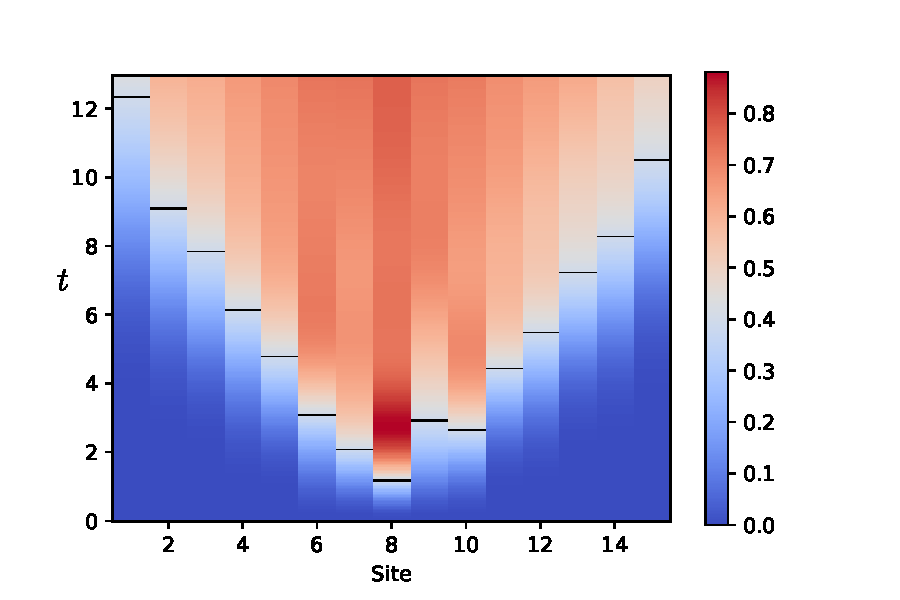
\includegraphics[width=\columnwidth]{colorplot}
	\caption{Illustration of the initially local operator. The bars indicate the time at which the OTOC passes 0.4, to emphasize the asymmetry.}
	\label{fig:colorplot}
\end{figure}

Asymmetric transport is seen in ``staircase" and ``glider" circuits, but we wanted to show it is also possible in time-independent Hamiltonians. 

In a 1-D circuit, how asymmetric can the spreading be?

On the edge of a 2-D system, spreading can be chiral even with a finite circuit depth~\cite{PoChiralCircuit}.

To be completely chiral with only 1 dimension, the circuit will have to be of infinite depth.

Given a constraint on the depth, how asymmetric can the spreading be?

In this paper we will start by discussing a local Hamiltonian with asymmetric spreading. We show that it is a general Hamiltonian, and provide multiple methods for measuring $v_B$ for left and right spreading. We then discuss staircase circuits in the small- and large-staircase limit and show that in the latter limit the circuit is completely chiral.

Throughout this paper we will use different methods to measure $v_B$. For the Hamiltonian system, we use two methods, both directly related to the spreading of operators. The first is non-local, measuring the velocity of the peak in the right- and left-weights. The other defines velocity-dependent Lyapunov exponents from the early-time OTOCs. For the circuit we extract $v_B$ from the growth rate of the entanglement entropy.

\tableofcontents

\section{Local Hamiltonians}

In order to define a local Hamiltonian with asymmetric spreading, we have to move away from 2-site interactions because these will have to be symmetric. The space of 3-site Hamiltonians is large ($q^{6} = 64$) so we restrict to SU(2)-symmetric terms.

This space is still large \charlie{Does it matter how large?}, but we know we want Hamiltonians that are different in opposite directions. If we restrict further to Hamiltonians antisymmetric under inversion of the spin chain, we are left with only one option, the triple product of spins. The Hamiltonian on the full chain is then
\begin{align}
H = \sum_{i=1}^{L-2}{\bf S}_i\cdot({\bf S}_{i+1}\times {\bf S}_{i+2})\nonumber
\end{align}

\subsection{Degeneracy and Generality}

As is, the model is not general, presenting a large degeneracy at $E=0$. This can be traced to the inversion antisymmetry, along with other related antisymmetries in the model~\cite{1710.05927}. \charlie{Should we go in-depth to show that various parts of the antisymmetry can be broken, etc?} We can fully break this degeneracy within each U(1) block by introducing a random field in the $Z$ direction, so the total Hamiltonians is
\begin{align}
H = \sum_{i=1}^{L-2}{\bf S}_i\cdot({\bf S}_{i+1}\times {\bf S}_{i+2}) + 
	\sum_{i=1}^{L}h_iS_i^z,
\end{align}
where each $h_i$ has a uniform probability distribution on $[-h,h]$. This field breaks the SU(2) symmetry but leaves the U(1) subgroup intact.

For sufficiently large $h$ the model becomes localized. In the large-$L$ limit the transition from ergodic to localized is a phase transition, described in~\cite{1010.1992v1}. The transition for the present model can be seen in Fig.~\ref{fig:levelrepultrans}, showing the ratio of adjacent energy gaps. Note that at smaller $L$ the model also drifts away from GUE statistics at very small $h$, when the field is no longer large enough to fully lift the $E=0$ degeneracy.

\begin{figure}
	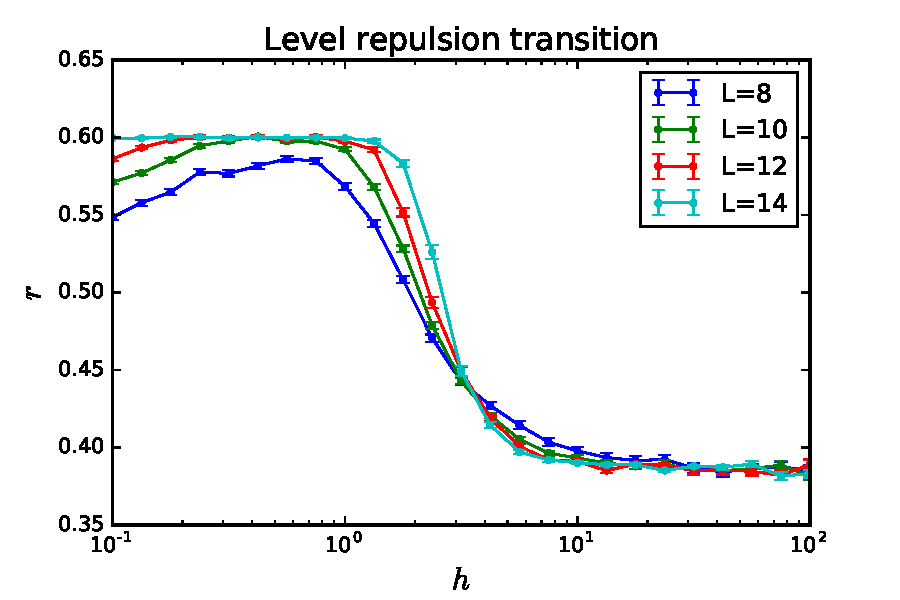
\includegraphics[width=\columnwidth]{levelrepultrans}
	\caption{Phase transition for the model, with level repulsion parameter plotted against field strength. Note that in the thermalizing phase the ratio is $~0.6$ instead of $0.53$ because the statistics are GUE instead of GOE. \charlie{I think I remember Vedika saying this but I can't find where.}}
	\label{fig:levelrepultrans}
\end{figure}

\subsection{Right-weight peaks}

We will measure the asymmetry using two metrics. The first is the weight of all operators with right (left) endpoint on site $i$, which we will call the right (left) weight. The other is the OTOC. \charlie{should we define these in this section?} \charlie{Make sure to point out use of initial operators as being on site 0 or $L-1$}.

We use the definition of the right weight from~\cite{KeyserlingkHydro2017}. An arbitrary operator $\cal O$ can be decomposed into Pauli strings ${\cal O} = \sum_\nu c_\nu \sigma^\nu$ where each string contains one of $\{I, X, Y, Z\}$ acting on each site. As the operator evolves in time, so do the $c_\nu$. The right weight is then
\begin{align}
\rho_r(i,t) = \sum_\nu\abs{c_\nu(t)}^2\delta(\text{RHS}(\nu) = i),
\end{align}
where the delta function ensures that we only count Pauli strings that have their right-most non-identity operator on site $i$. The left weight $\rho_l(i,t)$ is defined analogously.  If $\cal O$ is initially local on site $j$ then $\rho_r(i,0) = \rho_l(i,0) = \delta_{ij}$. As the operator spreads, the support of $\rho_r$ moves right at $v_{B,r}$ and $\rho_L$ moves left at $v_{B,l}$. Operator broadening manifests itself in the support of both weights increasing in size. At late times both weights should vanish near $j$.

In the thermalizing phase, the right weights peak as the information front passes. Because of the three-site nature of each term in the Hamiltonian, the right weight and OTOC exhibit an ``odd-even" effect. It is possible to account for these by averaging judiciously, or by only looking at even (or odd) sites. At $L=13$, there are enough even sites that the asymmetry can be seen. For a picture of the rights weights with their successive peaks, see Fig.~\ref{fig:Rweightpeakshape}. 

\begin{figure}
	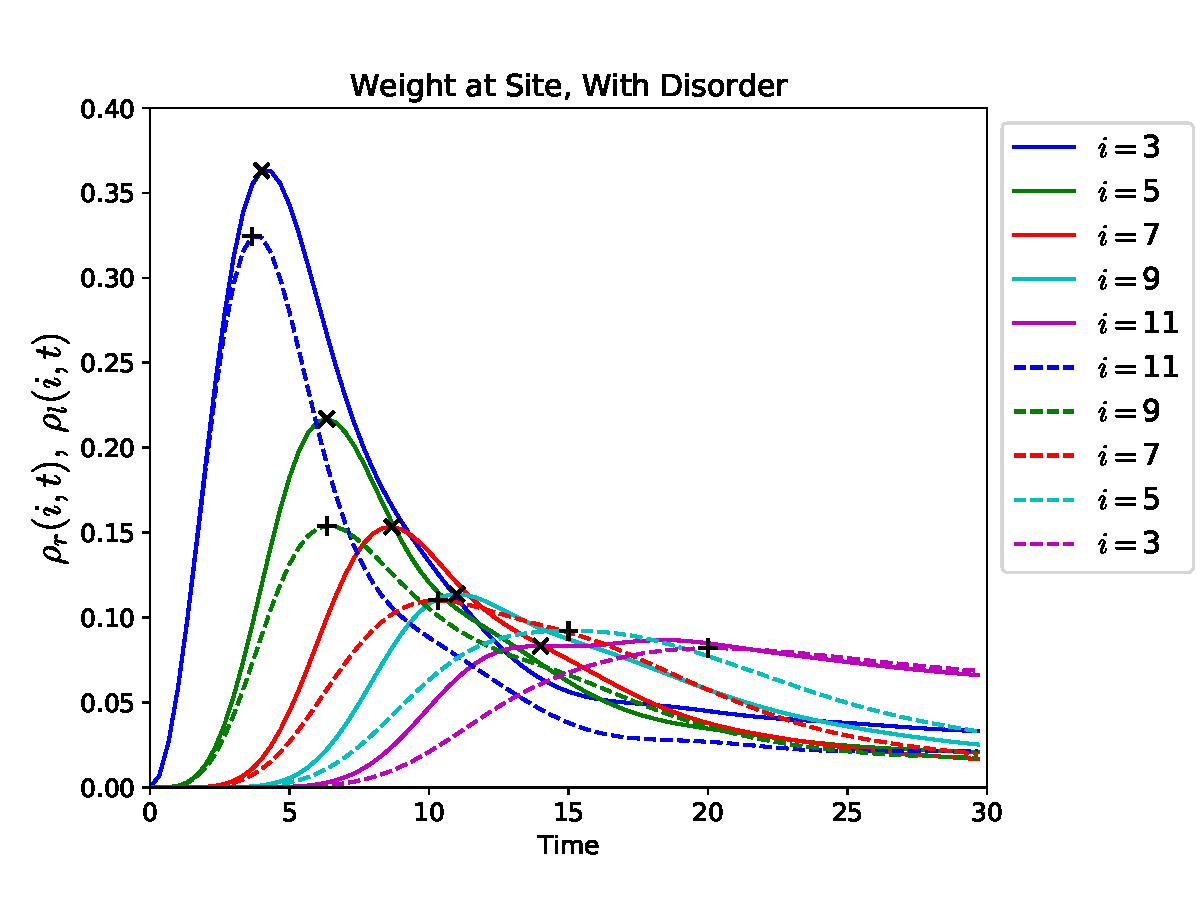
\includegraphics[width=\columnwidth]{Rweightpeakshape}
	\caption{Right weight at even sites for $L=13$. The peak travels ballistically. Later peaks are smaller \charlie{Is this due to broadening?}}
	\label{fig:Rweightpeakshape}
\end{figure}

Fig.~\ref{fig:Rweightpeaktimes} shows the peaks traveling ballistically. The peaks reach equivalent sites at later times for the left-moving wave, implying $v_{B,l}<v_{B,r}$. We can extract $v_{B,l}$ and $v_{B,r}$ from these curves by fitting linear functions to the peak timings.

\begin{figure}
	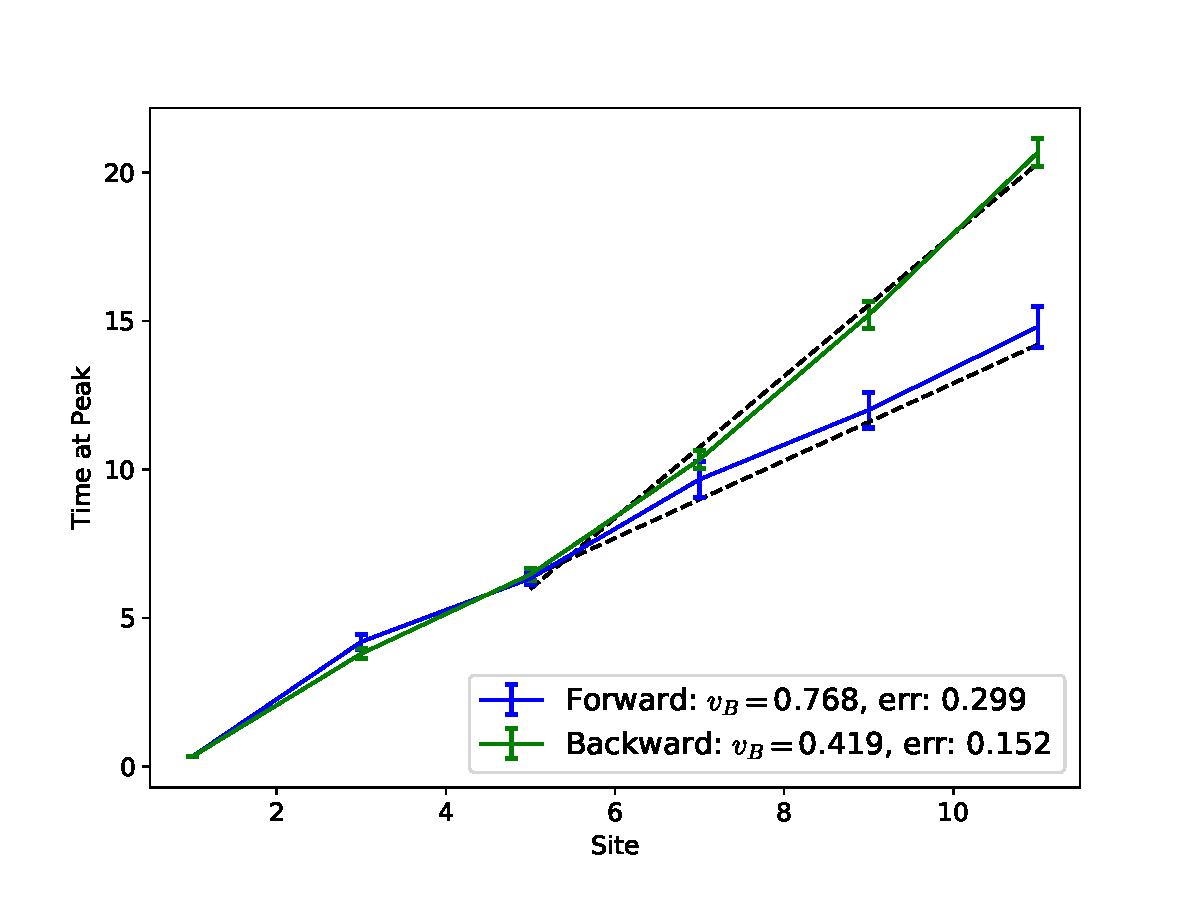
\includegraphics[width=\columnwidth]{Rweightpeaktimes}
	\caption{Time of peak vs. site. Since this is plot of time as a function of distance, the larger slope in the left weight means that $v_B$ is larger for propagation to the right. \charlie{This has the wrong normalization but I'm working on it.}}
	\label{fig:Rweightpeaktimes}
\end{figure}

\subsection{Velocity-dependent Lyapunov exponents}

It is also possible to extract butterfly velocities from the the velocity-dependent Lyapunov exponents, which in turn rely on the OTOC. We define the OTOC as 
\begin{align}
C(i,t) & = \half \langle|[Z_j(t),Z_i(0)]|^2\rangle_{\beta=0}\nonumber\\
&= 1 - \frac{1}{2^{L}}\Re\;\Tr\;[Z_j(t)Z_i(0)Z_j(t)Z_i(0)]
\end{align}
where $j$ is the site of the initial operator and the expectation value in the top row is with respect to a thermal ensemble at infinite temperature. We set $j=1$ to measure $v_{B,r}$ and $j=L$ to measure $v_{B,l}$. The OTOC should be order-1 inside the lightcone and exponentially small outside the lightcone defined by $v_B$.

From conservation of $\Sz$, the Hamiltonian and all relevant operators are block-diagonal, with the size of the $i^\text{th}$ block being $\binom{L}{i}$. For smaller blocks we can compute the trace directly, but for larger blocks this becomes computationally difficult. We then rely on quantum typicality to approximate the trace in the large blocks. For each disorder realization we replace the trace with an average over expectation values in pure states~\cite{Luitz2017}. The pure states are chosen Haar-randomly, and we find that using 5 vectors gives relative errors around 0.05 for all but the smallest blocks.

The VDLEs quantify how fast signals decay along constant-velocity trajectories outside the lightcone. In particular, if the OTOC is measured along the ray defined by each site $i$ at time $t_i = i/v$ for some $v$, then it should decay exponentially,
\begin{align}
	C(i, t) \sim e^{\lambda(v)t}\quad\text{for}\quad i = vt.
\end{align}
Ref.~\cite{khemani2018lambda} gives a thorough explanation of VDLEs. The name comes from the fact that the Lyapunov exponent defines how fast a signal grows inside a lightcone in a classically chaotic system.

In the current system, the OTOCs are influenced by the previously-mentioned odd-even effects. We can once again look only at even sites for sufficiently large $L$ to calculate $\lambda(v)$. Then $v_B$ is the point at which $\lambda(v)$ smoothly goes to 0.

Fig.~\ref{fig:vdle} shows the VDLEs for the right-going and left-going OTOCs. Finite-size effects slightly perturb $\lambda(v)$ around $v_B$, but we can see that $v_{B,l} \sim 0.7$ and $v_{B,r} \sim 0.85$.

\begin{figure}
	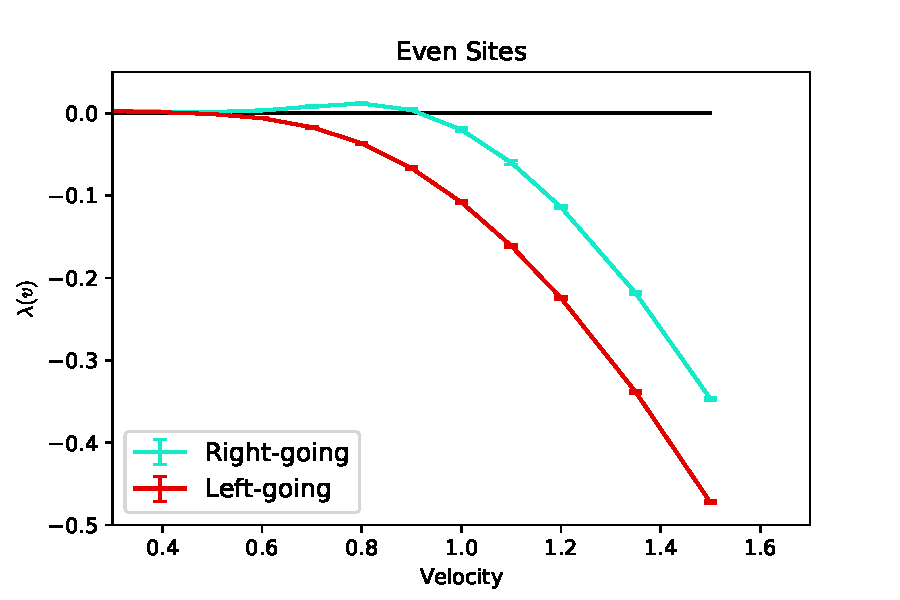
\includegraphics[width=\columnwidth]{vdle}
	\caption{Velocity-dependent Lyapunov exponents extracted from the OTOC on even sites. Since $\lambda_r(v)>\lambda_l(v)$, we know $v_{B,r}>v_{B,l}$.}
	\label{fig:vdle}
\end{figure}

\section{Circuit models} \label{sec:circ}

\charlie{I'm going to introduce the $\Gamma(s)$ formalism first and then staircase circuits, but I don't know if I should do it the other way around.}

Before discussing asymmetric circuits we will explain how $v_B$ can be extracted from the growth of entanglement. We will show that this method is particularly tractable in the large-$q$ limit before applying this method to staircase circuits. We will see that the butterfly velocities can be made arbitrarily asymmetric by considering long staircases.

Consider a spin chain of $N$ sites, each with dimension $q$. Sites are labeled by $i = 1,\dots, N$ , while the bonds between sites are labeled by $x = 1, \dots, N − 1$. Define the entropy function $S(x)$ as the bipartite entanglement entropy across bond $x$. 

After course-graining, the entanglement becomes a continuous function $S(x,t)$ with maximal slope 1. Given a circuit architecture, the entanglement growth rate is to first order only a function of the slope, so we can write \cite{jonay}
\begin{align}
\frac{\partial S}{\partial t} = \Gamma\left(\frac{\partial S}{\partial x}\right).
\end{align}
It is useful to define the entropy density $s = \partial S / \partial x$, which is so-called because the equilibrium entropy is $S(x, t) = s_\text{eq} \min\{x, L - x\}$. In our models $s_\text{eq} = 1$.

This function encodes the butterfly velocity as the derivative $\Gamma'(\partial S / \partial x)|_{s_\text{ext}}$, where $s_\text{ext}$ is either extremal entropy density. \charlie{Should we say why?} It follows that any symmetry $\Gamma(s)$ will have symmetric butterfly velocities. Then any circuit with asymmetric $\Gamma(s)$ will have asymmetric butterfly velocities.

\subsection{Staircase circuits}

Subadditivity tells us $|S(x + 1) - S(x)| \le S_1$, where $S_1$ is the entropy at a single site. If we take our logarithms with base $q$, then $S_1 \le 1$.

If a gate acts on bond $x$, it can increase the bipartite entanglement entropy $S(x)$, up to the constraint $|S(x + 1) - S(x)| \le 1$. In the large-$q$ limit, a Haar-randomly chosen gate will, with probability 1, maximally increase the entanglement across the bond it acts on~\cite{nahum2017quantum}. Given the previous constraint, this means that if a gate acts at bond $x$ at time $t$, then $S(x, t+1) = \min\left\lbrace S(x-1,t)+1, S(x+1,t)+1\right\rbrace$. \charlie{Should we explain why?} It suffices to consider integer-valued $S(x)$ with $|S(x)-S(x-1)|=1$ for all $x$. 

Staircase circuits of length $n$ are defined by always having strings of $n$ gates act on sites $x$ through $x+n-1$ in succession. For $n=1$ this is just a random architecture, but large $n$ results in more asymmetric circuits. \charlie{Would a figure of the staircase circuit, as in Fig. 38 or 39 in my thesis?}

\subsection{Asymmetric $v_B$}

For small $n$, we can simulate the circuit directly. For the growth rate curves of $n$-stair circuits for $n\le 6$ see Fig.~\ref{fig:compareRates}. 
\begin{figure}
	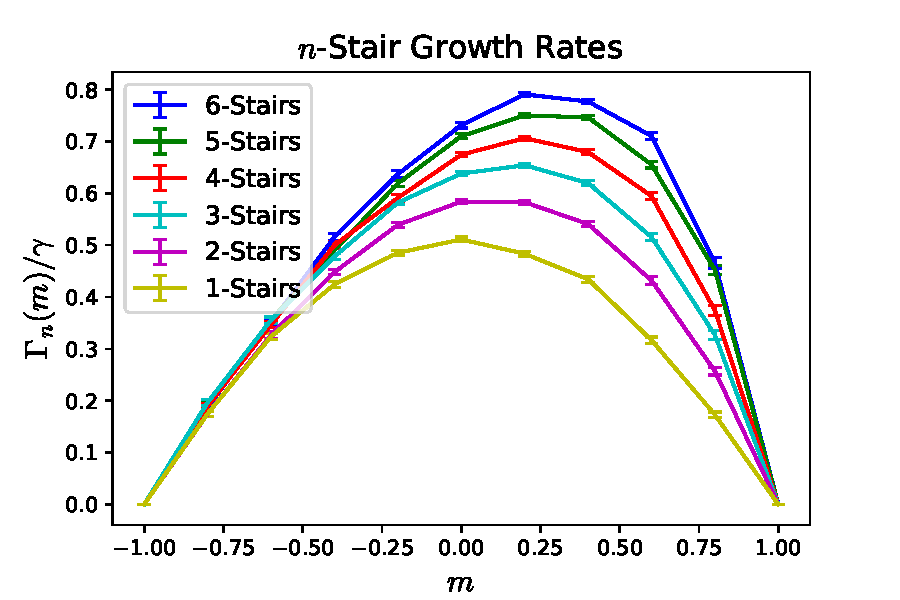
\includegraphics[width=\columnwidth]{compareRates.pdf}
	\caption{Empirical growth rate as a function of slope for $n$-stair circuits. The right/forward and left/backward butterfly velocities are the slopes of these curves at their endpoint, indicating that as the left $v_B$ stays constant, the right $v_B$ increases. The appendix includes an argument that the right $v_B$ is unbounded in the large-$n$ limit.}
	\label{fig:compareRates}
\end{figure}	
It is possible to approximate these growth rates by assuming the up and down steps are uncorrelated. Then the probability that a randomly placed gate will result in growth is $(1-s^2)/2$. Any asymmetry comes from the fact that for longer staircases, a gate acting on site $x$ is more likely to have been preceded by a gate on site $x-1$ so the step from $x-1$ to $x$ is more likely to be a down step.

Under these assumptions the growth rate is
\begin{align}
\Gamma_n(s) = \frac{\gamma}{n}\frac{1+s}{1-s}\bigg(
	(1+s)&\left[\left(\frac{1+s}{2}^2\right)^n-1\right]\nonumber \\
	&+n(1-s)\bigg). \label{eqn:growthrate}
\end{align}
This produces successively more asymmetric growth rates as $n$ increases. However, the correlation in the true steady state, and therefore the error of this approximation, also increases. It is possible to correct for the correlation term-by-term in correlation length, but this quickly becomes tedious. For 2-stairs, including the nearest-neighbor correlation removes most of the error in $\Gamma(s)$.

Luckily, as $n$ becomes very large or approaches the size of the system, the correlations again become unimportant. To see this we can consider the growth rate at $s = -1, 0,$ and 1.

The growth rate approaches $\Gamma_\infty = \gamma(s+1)$, so that for spreading to the left $v_B=1$ and for spreading to the right $v_B=\infty$. This is of course maximally asymmetric. 

\section{Conclusion}

Advantages of this model:
Time-independent Hamiltonian.
Only ingredients are chains of two-level systems.

Further work:
How do the velocities depend on $h$?
What happens at the phase transition?
Maximally asymmetric three-site Hamiltonians?
2-D systems?

%We'll want to cite a bunch of people~\cite{Larkinotoc,Lieb72,KitaevSYK,chaosbound,HosurYoshida,ShenkerStanfordButterfly,LocalizedShocks,CotlerRM,RobertsStanford,GuQiStanford,GuQi_rcft,StanfordWeakCoupling,PatelDiffusiveMetal,ChowdhuryON,Galitski_lyapunov,DoraMoessner,LuitzScrambling,ProsenWeakChaos,AleinerOTOC,MotrunichTFIM_otoc,FradkinHuse,ChalkerFloquetChaos,FawziScrambling,opspreadAdam, opspreadCurt, TiborCons, KhemaniCons}.

\section*{Acknowledgements}
We thank many people.

\charlie{Note somewhere about arXiv:1809.02614v1}

\bibliography{global}

\begin{appendix}


\end{appendix}

\end{document}
